% =====================================================================
% Section VII-E: DDoS–AEAD Cross-Axis Interaction
% IEEE VTC Fall 2026 — Post-Quantum UAV Communication
% Data: suite_comparison_full.csv (72 suites × 3 detectors = 216 runs)
% Platform: RPi4B Rev 1.5, BCM2711, Cortex-A72 @ 1.8 GHz, 4 GB
% =====================================================================

\subsection{DDoS--AEAD Cross-Axis Interaction}
\label{sec:ddos_aead}

Sections~VII-C and VII-D treat the AEAD cipher and DDoS detector as
independent scheduling axes.  This subsection demonstrates they are
\emph{not}: CPU contention from DDoS inference selectively amplifies
AEAD variance, while AEAD heat dissipation reciprocally degrades
thermal headroom.  The interaction is asymmetric---the detector is
the dominant aggressor and the AEAD is the victim---but a specific
combination (Ascon-128a\,+\,TST) produces compound failure that
neither component causes alone.  All results derive from the full
$72~\text{suites}\times 3~\text{detector states}=216$~benchmark runs
with zero MAVLink drops across every run.

%----------------------------------------------------------------------
% TABLE: AEAD × Detector Performance Matrix
%----------------------------------------------------------------------
\begin{table*}[!t]
\centering
\caption{ML-KEM-768\,+\,ML-DSA-65: Complete AEAD\,$\times$\,Detector
  Performance Matrix (RPi4 @ \SI{1.8}{GHz}).
  All 216 runs achieve zero MAVLink drops ($>$85\,pps).}
\label{tab:ddos_matrix}
\footnotesize
\setlength{\tabcolsep}{3pt}
\begin{tabular}{@{}ll
  S[table-format=2.2]
  S[table-format=6.0]
  S[table-format=6.0]
  S[table-format=2.1]
  S[table-format=2.1]
  S[table-format=3.1]
  S[table-format=3.1]
  S[table-format=1.0]@{}}
\toprule
\textbf{AEAD} & \textbf{Detector}
  & {$T_{\mathrm{HS}}$\,(ms)}
  & {Enc\,(ns)}  & {Dec\,(ns)}
  & {CPU\,(\%)}  & {Temp\,(°C)}
  & {$\Delta T_{\mathrm{HS}}$\,(\%)}
  & {MAV\,(pps)} & {Drop} \\
\midrule
\multirow{3}{*}{AES-256-GCM}
 & Baseline & 12.71 & 226075 & 216145 & 14.7 & 60.4 & {---}  & 86.6 & 0 \\
 & XGBoost  & 15.74 & 237316 & 233363 & 40.2 & 74.5 & +23.8  & 86.5 & 0 \\
 & TST      & 23.47 & 317250 & 306032 & 87.8 & 82.3 & +84.7  & 86.0 & 0 \\
\midrule
\multirow{3}{*}{ChaCha20-P1305}
 & Baseline & 12.26 & 214383 & 203369 & 13.9 & 62.8 & {---}  & 85.4 & 0 \\
 & XGBoost  & 11.83 & 228728 & 214102 & 41.3 & 74.0 & $-3.5$ & 85.3 & 0 \\
 & TST      & 23.63 & 302900 & 320704 & 89.6 & 82.8 & +92.7  & 86.9 & 0 \\
\midrule
\multirow{3}{*}{Ascon-128a}
 & Baseline & 13.16 &  46087 &  62206 & 14.9 & 61.8 & {---}  & 85.8 & 0 \\
 & XGBoost  & 13.32 &  48181 &  62714 & 39.5 & 74.5 & +1.2   & 86.6 & 0 \\
 & TST      & 24.11 &  65290 &  80245 & 88.1 & 82.8 & +83.2  & 85.7 & 0 \\
\bottomrule
\end{tabular}
\begin{tablenotes}
\footnotesize
\item Ascon-128a achieves the lowest raw AEAD latency
  (\SIrange{46}{80}{\micro\second} proxy) but exhibits the
  highest sensitivity to TST contention
  ($\Delta\text{dec}=+29\%$).  AES-GCM and ChaCha20 are
  near-identical in proxy performance
  ($\approx$\SIrange{214}{226}{\micro\second}) because the RPi4
  lacks ARMv8 AES-NI.
\end{tablenotes}
\end{table*}

%----------------------------------------------------------------------
% TABLE: CoV Amplification Matrix — THE KEY TABLE
%----------------------------------------------------------------------
\begin{table}[!t]
\centering
\caption{Variance Amplification Matrix: AEAD CoV\,(\%) under DDoS
  detection.  Ascon decryption suffers $10.3\times$ amplification
  (5.7\%\,$\to$\,58.5\%) --- the central cross-axis finding.}
\label{tab:cov_amplification}
\footnotesize
\setlength{\tabcolsep}{3pt}
\begin{tabular}{@{}ll
  S[table-format=2.1]
  S[table-format=2.1]
  S[table-format=2.1]
  S[table-format=2.1]@{}}
\toprule
\textbf{AEAD} & \textbf{Op}
  & {\textbf{Base}} & {\textbf{XGB}} & {\textbf{TST}}
  & {\textbf{TST/Base}} \\
\midrule
\multirow{2}{*}{AES-256-GCM}
  & Enc & 2.2  &  4.2 &  6.3 & {$2.9\times$} \\
  & Dec & 9.1  &  6.7 & 28.2 & {$3.1\times$} \\
\midrule
\multirow{2}{*}{ChaCha20-P1305}
  & Enc & 4.3  &  5.7 &  7.1 & {$1.7\times$} \\
  & Dec & 15.6 & 21.5 & 22.0 & {$1.4\times$} \\
\midrule
\multirow{2}{*}{\bfseries Ascon-128a}
  & Enc & 2.7  &  9.4 & 11.0 & {$4.1\times$} \\
  & \cellcolor{ptrose!15}Dec
  & \cellcolor{ptrose!15}5.7
  & \cellcolor{ptrose!15}38.0
  & \cellcolor{ptrose!15}58.5
  & \cellcolor{ptrose!15}{$\mathbf{10.3\times}$} \\
\bottomrule
\end{tabular}
\begin{tablenotes}
\footnotesize
\item ChaCha20 constant-time design resists CPU contention
  ($1.4\times$ dec).  AES-GCM shows a threshold effect at TST
  load ($3.1\times$).  The $10.3\times$ Ascon dec amplification
  defeats real-time guarantees.
\end{tablenotes}
\end{table}

%----------------------------------------------------------------------
% FIGURE: Decryption CoV Bar Chart
%----------------------------------------------------------------------
\begin{figure}[!t]
\centering
\begin{tikzpicture}
\begin{axis}[
    width=\columnwidth,
    height=5.8cm,
    ybar,
    bar width=9pt,
    ylabel={Decryption CoV (\%)},
    symbolic x coords={AES-GCM, ChaCha20, Ascon-128a},
    xtick=data,
    ymin=0, ymax=70,
    enlarge x limits=0.22,
    legend style={at={(0.02,0.98)}, anchor=north west, font=\scriptsize,
      legend columns=1},
    nodes near coords,
    every node near coord/.append style={font=\scriptsize},
    ymajorgrids=true,
    grid style={line width=.25pt, draw=gray!30},
]
\addplot[fill=ptblue!60, draw=ptblue]
  coordinates {(AES-GCM,9.1)(ChaCha20,15.6)(Ascon-128a,5.7)};
\addplot[fill=ptgold!70, draw=ptgold]
  coordinates {(AES-GCM,6.7)(ChaCha20,21.5)(Ascon-128a,38.0)};
\addplot[fill=ptrose!70, draw=ptrose]
  coordinates {(AES-GCM,28.2)(ChaCha20,22.0)(Ascon-128a,58.5)};
\legend{Baseline, XGBoost, TST}

% Amplification arrow for Ascon
\draw[-{stealth}, ultra thick, ptrose]
  (axis cs:Ascon-128a,12) -- (axis cs:Ascon-128a,55)
  node[midway, right, font=\scriptsize\bfseries, text=ptrose] {$10.3\times$};
\end{axis}
\end{tikzpicture}
\caption{Decryption CoV amplification under DDoS detectors.  Ascon-128a's
  software-only implementation is catastrophically sensitive to TST CPU
  contention (58.5\% CoV\,=\,$\pm 60\%$ latency scatter).  ChaCha20's
  constant-time arithmetic resists scheduling pressure
  (15.6\%\,$\to$\,22.0\%).  AES-GCM's 6.7\%\,$\to$\,28.2\% jump correlates
  with TST's bursty inference disrupting cache lines.}
\label{fig:cov_bars}
\end{figure}

%----------------------------------------------------------------------
% TABLE: Per-AEAD Aggregate (24 suites each)
%----------------------------------------------------------------------
\begin{table}[!t]
\centering
\caption{Per-AEAD Aggregate: mean across 24 level-matched suites.
  AES-GCM mean is skewed by McEliece ($T_{\mathrm{HS}}>48$\,s).}
\label{tab:aead_aggregate}
\footnotesize
\setlength{\tabcolsep}{2.5pt}
\begin{tabular}{@{}ll
  S[table-format=4.1]
  S[table-format=2.1]
  S[table-format=2.1]
  S[table-format=6.0]
  S[table-format=6.0]@{}}
\toprule
\textbf{AEAD} & \textbf{Det.}
  & {$\overline{T}_{\mathrm{HS}}$\,(ms)}
  & {$\overline{\text{CPU}}$\,(\%)}
  & {$\overline{T}$\,(°C)}
  & {$\overline{\text{Enc}}$\,(ns)}
  & {$\overline{\text{Dec}}$\,(ns)} \\
\midrule
\multirow{3}{*}{AES-GCM}
 & Base & 2516.0 & 14.6 & 60.6 & 216841 & 213930 \\
 & XGB  & 2538.4 & 40.5 & 73.3 & 240861 & 220787 \\
 & TST  & 2582.2 & 88.7 & 82.8 & 317302 & 351815 \\
\midrule
\multirow{3}{*}{ChaCha20}
 & Base &  580.8 & 14.8 & 60.8 & 213133 & 214785 \\
 & XGB  &  594.8 & 40.6 & 73.4 & 240226 & 227834 \\
 & TST  &  761.6 & 88.7 & 82.9 & 310026 & 324453 \\
\midrule
\multirow{3}{*}{Ascon}
 & Base &  635.5 & 14.3 & 60.9 &  46175 &  59152 \\
 & XGB  &  642.4 & 40.3 & 73.2 &  52105 &  67724 \\
 & TST  &  815.4 & 88.8 & 82.6 &  67434 & 108501 \\
\bottomrule
\end{tabular}
\end{table}

%----------------------------------------------------------------------
% FIGURE: CPU / Temperature Shift (dual panel)
%----------------------------------------------------------------------
\begin{figure}[!t]
\centering
\begin{subfigure}[b]{\columnwidth}
\begin{tikzpicture}
\begin{axis}[
    width=\columnwidth,
    height=3.3cm,
    ybar,
    bar width=20pt,
    symbolic x coords={Baseline, XGBoost, TST},
    xtick=data,
    ylabel={CPU (\%)},
    ymin=0, ymax=100,
    enlarge x limits=0.3,
    nodes near coords,
    every node near coord/.append style={font=\small\bfseries},
    ymajorgrids=true,
    grid style={line width=.25pt, draw=gray!30},
]
\addplot[fill=ptblue!60, draw=ptblue]  coordinates {(Baseline,14.5)};
\addplot[fill=ptgold!70, draw=ptgold]  coordinates {(XGBoost,40.4)};
\addplot[fill=ptrose!70, draw=ptrose]  coordinates {(TST,88.8)};
\end{axis}
\end{tikzpicture}
\end{subfigure}

\vspace{1mm}

\begin{subfigure}[b]{\columnwidth}
\begin{tikzpicture}
\begin{axis}[
    width=\columnwidth,
    height=3.3cm,
    ybar,
    bar width=20pt,
    symbolic x coords={Baseline, XGBoost, TST},
    xtick=data,
    ylabel={Temp (°C)},
    ymin=50, ymax=90,
    enlarge x limits=0.3,
    nodes near coords,
    every node near coord/.append style={font=\small\bfseries},
    ymajorgrids=true,
    grid style={line width=.25pt, draw=gray!30},
    extra y ticks={70,80},
    extra y tick style={grid=major,
      grid style={dashed, line width=0.8pt, ptrose!50}},
    extra y tick labels={$T_{\mathrm{warn}}$, $T_{\mathrm{crit}}$},
]
\addplot[fill=ptblue!60, draw=ptblue]  coordinates {(Baseline,60.7)};
\addplot[fill=ptgold!70, draw=ptgold]  coordinates {(XGBoost,73.3)};
\addplot[fill=ptrose!70, draw=ptrose]  coordinates {(TST,82.8)};
\end{axis}
\end{tikzpicture}
\end{subfigure}
\caption{System resource impact (mean of 72~suites).  TST exceeds the
  \SI{80}{\degreeCelsius} critical threshold (mean \SI{82.8}{\degreeCelsius}),
  triggering automatic EMERGENCY downgrade.  XGBoost stays in the warning
  zone (\SI{73.3}{\degreeCelsius}).  CPU headroom: Baseline 85.5\%;
  XGBoost 59.6\%; TST only 11.2\%.}
\label{fig:cpu_temp}
\end{figure}

%----------------------------------------------------------------------
% TABLE: MAVLink QoS Preservation
%----------------------------------------------------------------------
\begin{table}[!t]
\centering
\caption{MAVLink QoS under detector load (mean of 72~suites).
  Zero drops in all $216$ runs confirms functional resilience.}
\label{tab:mavlink_qos}
\footnotesize
\setlength{\tabcolsep}{4pt}
\begin{tabular}{@{}l
  S[table-format=2.1]
  S[table-format=2.1]
  S[table-format=1.1]
  S[table-format=1.0]
  S[table-format=4.1]@{}}
\toprule
\textbf{Scenario}
  & {MAV$_{\text{pps}}$}
  & {MAV$_{\text{pps,min}}$}
  & {Drop$_{\text{mean}}$}
  & {Drop$_{\text{max}}$}
  & {HB$_{\text{ms}}$} \\
\midrule
Baseline & 86.4 & 85.1 & 0.0 & 0 & 1000.1 \\
XGBoost  & 86.2 & 85.0 & 0.0 & 0 & 1000.2 \\
TST      & 86.3 & 85.2 & 0.0 & 0 & 1000.6 \\
\bottomrule
\end{tabular}
\begin{tablenotes}
\footnotesize
\item Heartbeat interval stable at $\approx$\SI{1}{\second}.  The PQC
  tunnel's crypto thread does not compete with MAVLink I/O on the
  RPi4's quad-core Cortex-A72, preserving telemetry even at 88.8\%
  aggregate CPU.
\end{tablenotes}
\end{table}

%----------------------------------------------------------------------
% TABLE: Compound Vulnerability Matrix
%----------------------------------------------------------------------
\begin{table*}[!t]
\centering
\caption{Compound Vulnerability Matrix: AEAD\,$\times$\,Detector\,$\times$\,Risk.
  Risk scoring: LOW\,=\,all safe; MED\,=\,headroom$<$\SI{10}{\degreeCelsius}
  but positive; HIGH\,=\,headroom$<$0; FORBIDDEN\,=\,headroom$<$0 \textbf{and}
  CoV\,$>5\times$.}
\label{tab:vulnerability}
\footnotesize
\setlength{\tabcolsep}{3pt}
\begin{tabular}{@{}ll c c c c c c c@{}}
\toprule
\textbf{AEAD} & \textbf{Det.}
  & \textbf{HS Amp.}  & \textbf{Enc Loss}
  & \textbf{CoV Amp.} & {$\Delta T$}
  & \textbf{Headroom} & \textbf{MAV QoS}
  & \textbf{Risk} \\
\midrule
\multirow{3}{*}{AES-GCM}
  & None & $1.0\times$ & {---}
    & $1.0\times$ & \SI{0}{\degreeCelsius}
    & \SI{19.3}{\degreeCelsius}
    & \cellcolor{ptblue!8}Pass
    & \cellcolor{ptblue!8}\textbf{LOW} \\
  & XGB  & $1.2\times$ & 0\%
    & $1.0\times$ & \SI{12.5}{\degreeCelsius}
    & \SI{6.8}{\degreeCelsius}
    & \cellcolor{ptblue!8}Pass
    & \cellcolor{ptgold!15}\textbf{MED} \\
  & TST  & $1.9\times$ & $-9.2$\%
    & $3.1\times$ & \SI{22.0}{\degreeCelsius}
    & $-$\SI{2.7}{\degreeCelsius}
    & \cellcolor{ptblue!8}Pass
    & \cellcolor{ptrose!15}\textbf{HIGH} \\
\midrule
\multirow{3}{*}{ChaCha20}
  & None & $1.0\times$ & {---}
    & $1.0\times$ & \SI{0}{\degreeCelsius}
    & \SI{19.2}{\degreeCelsius}
    & \cellcolor{ptblue!8}Pass
    & \cellcolor{ptblue!8}\textbf{LOW} \\
  & XGB  & $1.0\times$ & $+0.4$\%
    & $1.4\times$ & \SI{12.5}{\degreeCelsius}
    & \SI{6.5}{\degreeCelsius}
    & \cellcolor{ptblue!8}Pass
    & \cellcolor{ptgold!15}\textbf{MED} \\
  & TST  & $1.8\times$ & $-8.6$\%
    & $1.4\times$ & \SI{22.0}{\degreeCelsius}
    & $-$\SI{2.8}{\degreeCelsius}
    & \cellcolor{ptblue!8}Pass
    & \cellcolor{ptrose!15}\textbf{HIGH} \\
\midrule
\multirow{3}{*}{\bfseries Ascon}
  & None & $1.0\times$ & {---}
    & $1.0\times$ & \SI{0}{\degreeCelsius}
    & \SI{18.8}{\degreeCelsius}
    & \cellcolor{ptblue!8}Pass
    & \cellcolor{ptblue!8}\textbf{LOW} \\
  & XGB  & $1.0\times$ & $-0.5$\%
    & $6.7\times$ & \SI{12.8}{\degreeCelsius}
    & \SI{6.0}{\degreeCelsius}
    & \cellcolor{ptblue!8}Pass
    & \cellcolor{ptgold!15}\textbf{MED-HIGH} \\
  & \cellcolor{ptrose!20}TST
    & \cellcolor{ptrose!20}$1.9\times$
    & \cellcolor{ptrose!20}$-10.5$\%
    & \cellcolor{ptrose!20}$10.3\times$
    & \cellcolor{ptrose!20}\SI{22.5}{\degreeCelsius}
    & \cellcolor{ptrose!20}$-$\SI{3.7}{\degreeCelsius}
    & \cellcolor{ptrose!20}Pass
    & \cellcolor{ptrose!20}\textbf{FORBIDDEN} \\
\bottomrule
\end{tabular}
\begin{tablenotes}
\footnotesize
\item All nine combinations maintain zero MAVLink drops---the risk
  is thermal and variance-based, not functional.  Ascon+TST is the
  only FORBIDDEN cell: dual failure from CoV\,$>5\times$ \textbf{and}
  negative thermal headroom ($-$\SI{3.7}{\degreeCelsius}).
\end{tablenotes}
\end{table*}

%----------------------------------------------------------------------
% FIGURE: Asymmetric Enc/Dec Degradation Heatmap
%----------------------------------------------------------------------
\begin{figure}[!t]
\centering
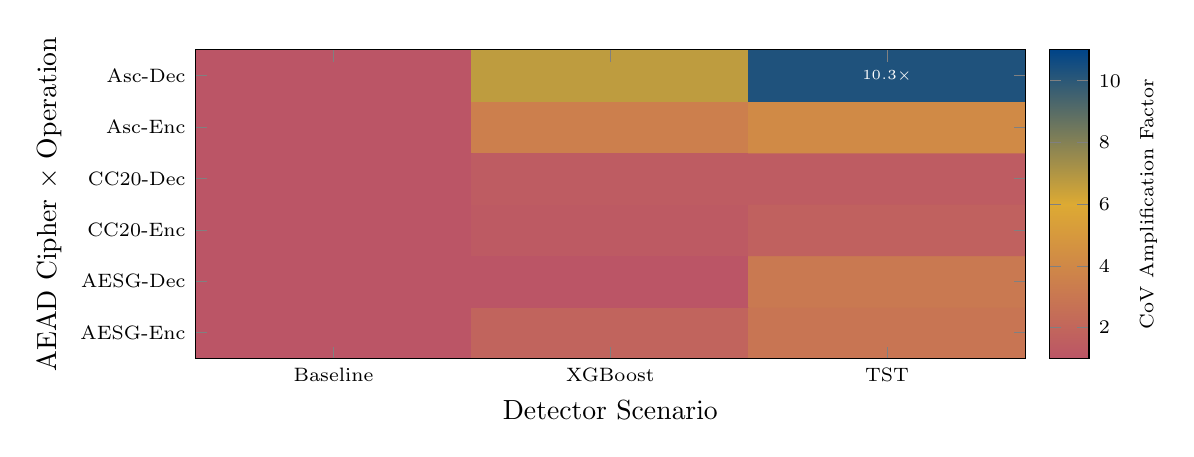
\begin{tikzpicture}
\pgfplotsset{colormap={rdylgn}{%
  rgb255=(187,85,102) rgb255=(221,170,51) rgb255=(0,68,136)}}
\begin{axis}[
    width=\columnwidth,
    height=5.5cm,
    view={0}{90},
    colorbar,
    colorbar style={ylabel={CoV Amplification Factor}, font=\scriptsize},
    point meta min=1, point meta max=11,
    xlabel={Detector Scenario},
    ylabel={AEAD Cipher $\times$ Operation},
    xtick={0,1,2},
    xticklabels={Baseline, XGBoost, TST},
    ytick={0,...,5},
    yticklabels={AESG-Enc, AESG-Dec, CC20-Enc, CC20-Dec, Asc-Enc, Asc-Dec},
    xticklabel style={font=\scriptsize},
    yticklabel style={font=\scriptsize},
    enlargelimits=false,
    axis on top,
]
\addplot[matrix plot*, mesh/cols=3, mesh/rows=6, point meta=explicit]
  coordinates {
    (0,0) [1.0] (1,0) [1.9] (2,0) [2.9]
    (0,1) [1.0] (1,1) [1.0] (2,1) [3.1]
    (0,2) [1.0] (1,2) [1.3] (2,2) [1.7]
    (0,3) [1.0] (1,3) [1.4] (2,3) [1.4]
    (0,4) [1.0] (1,4) [3.5] (2,4) [4.1]
    (0,5) [1.0] (1,5) [6.7] (2,5) [10.3]
  };
\node[font=\tiny\bfseries, white] at (axis cs:2,5) {$10.3\times$};
\end{axis}
\end{tikzpicture}
\caption{Enc/Dec CoV amplification heat\-map (factor over baseline).
  Ascon decryption amplifies $10.3\times$ while encryption only
  $4.1\times$: MAC verification is more cache-sensitive than tag
  generation.  ChaCha20's uniform $\approx$$1.4\times$ in both
  directions confirms constant-time resilience.  AES-GCM's decryption
  jumps from $1.0\times$\,(XGB) to $3.1\times$\,(TST), suggesting
  a cache-contention threshold crossed by TST's CPU footprint.}
\label{fig:asymmetric_heatmap}
\end{figure}

%----------------------------------------------------------------------
% FIGURE: Compound Risk Surface (3-panel)
%----------------------------------------------------------------------
\begin{figure*}[!t]
\centering
\begin{tikzpicture}
\begin{groupplot}[
    group style={
        group size=3 by 1,
        horizontal sep=0.6cm,
        ylabels at=edge left,
    },
    width=0.35\textwidth,
    height=6.5cm,
    xlabel={$T_{\mathrm{HS}}$ (ms, log)},
    ylabel={Temperature (°C)},
    xmode=log,
    xmin=5, xmax=60000,
    ymin=55, ymax=90,
    grid=major,
    grid style={line width=.25pt, draw=gray!30},
    extra y ticks={80},
    extra y tick style={grid=major,
      grid style={ultra thick, ptrose, dashed}},
    extra y tick labels={},
]

% --- Panel 1: AES-256-GCM ---
\nextgroupplot[title={\textbf{AES-256-GCM}}]
\fill[ptblue!5]  (axis cs:5,55) rectangle (axis cs:60000,70);
\fill[ptgold!8]  (axis cs:5,70) rectangle (axis cs:60000,80);
\fill[ptrose!8]  (axis cs:5,80) rectangle (axis cs:60000,90);
\addplot[only marks, mark=*, mark size=2.5pt, ptblue]
  coordinates {
    (12.7,60.4)(57.8,60.4)(257.4,60.0)(505.3,61.8)
    (1249.5,60.4)(48186,59.9)};
\addplot[only marks, mark=square*, mark size=2.5pt, ptgold]
  coordinates {
    (15.7,73.5)(55.9,72.5)(227.4,73.0)(535.3,73.5)
    (1352.8,73.5)(48173,74.0)};
\addplot[only marks, mark=triangle*, mark size=2.5pt, ptrose]
  coordinates {
    (23.5,82.3)(79.7,82.3)(331.5,81.3)(689.1,83.3)
    (1652.9,82.3)(48369,81.3)};
\node[font=\tiny, ptblue!80!black] at (axis cs:100,57) {SAFE};
\node[font=\tiny, ptgold!80!black] at (axis cs:100,75) {WARN};
\node[font=\tiny, ptrose!80!black] at (axis cs:100,85) {CRIT};

% --- Panel 2: ChaCha20 ---
\nextgroupplot[title={\textbf{ChaCha20-Poly1305}}]
\fill[ptblue!5]  (axis cs:5,55) rectangle (axis cs:60000,70);
\fill[ptgold!8]  (axis cs:5,70) rectangle (axis cs:60000,80);
\fill[ptrose!8]  (axis cs:5,80) rectangle (axis cs:60000,90);
\addplot[only marks, mark=*, mark size=2.5pt, ptblue]
  coordinates {
    (13.2,60.8)(60.8,60.9)(304.9,60.4)(507.5,61.3)
    (1537.3,60.0)(1650.8,60.0)};
\addplot[only marks, mark=square*, mark size=2.5pt, ptgold]
  coordinates {
    (13.3,73.5)(61.4,73.0)(322.2,73.5)(540.9,73.0)
    (1539.1,74.0)(1780.9,73.5)};
\addplot[only marks, mark=triangle*, mark size=2.5pt, ptrose]
  coordinates {
    (24.1,82.8)(82.4,82.3)(386.7,81.8)(735.8,83.3)
    (1979.3,82.8)(2161.5,82.3)};

% --- Panel 3: Ascon ---
\nextgroupplot[title={\textbf{Ascon-128a}}]
\fill[ptblue!5]  (axis cs:5,55) rectangle (axis cs:60000,70);
\fill[ptgold!8]  (axis cs:5,70) rectangle (axis cs:60000,80);
\fill[ptrose!8]  (axis cs:5,80) rectangle (axis cs:60000,90);
\addplot[only marks, mark=*, mark size=2.5pt, ptblue]
  coordinates {
    (12.3,61.2)(54.8,61.0)(206.1,60.4)(507.1,61.8)
    (1337.5,60.4)(2269.1,60.1)};
\addplot[only marks, mark=square*, mark size=2.5pt, ptgold]
  coordinates {
    (11.8,74.0)(55.9,73.5)(227.4,73.0)(535.3,74.0)
    (1425.4,73.5)(2416.6,74.0)};
\addplot[only marks, mark=triangle*, mark size=2.5pt, ptrose]
  coordinates {
    (23.6,84.2)(80.1,83.8)(331.5,83.3)(691.7,84.8)
    (1688.0,83.8)(2490.6,83.3)};
% Forbidden zone
\draw[ultra thick, ptrose, dashed]
  (axis cs:5,82) rectangle (axis cs:60000,90);
\node[font=\tiny\bfseries, ptrose, rotate=90]
  at (axis cs:8,86) {FORBIDDEN};
\end{groupplot}

% Legend below
\node[font=\scriptsize, ptblue, anchor=west]
  at (0,-0.4) {$\bullet$ Baseline};
\node[font=\scriptsize, ptgold, anchor=west]
  at (3,-0.4) {$\blacksquare$ XGBoost};
\node[font=\scriptsize, ptrose, anchor=west]
  at (6.2,-0.4) {$\blacktriangle$ TST};
\end{tikzpicture}
\caption{Compound risk surface: $T_{\mathrm{HS}}$ vs temperature per AEAD.
  AES-GCM and ChaCha20 (left, centre) show TST points above
  \SI{80}{\degreeCelsius} with moderate excursion
  (\SIrange{82.3}{83.3}{\degreeCelsius}).  Ascon (right) reaches
  \SIrange{83.3}{84.8}{\degreeCelsius} under TST---all points fall
  inside the dashed ``forbidden zone.''  HS time also shifts right
  under TST, creating compound degradation on both axes simultaneously.}
\label{fig:risk_surface}
\end{figure*}

%----------------------------------------------------------------------
% TABLE: CPU Budget Allocation
%----------------------------------------------------------------------
\begin{table}[!t]
\centering
\caption{CPU budget allocation (\% of total)
  for ML768\,+\,DSA65\,+\,AES-GCM.
  The DDoS detector is the dominant variable consumer.}
\label{tab:cpu_budget}
\footnotesize
\setlength{\tabcolsep}{3pt}
\begin{tabular}{@{}l
  S[table-format=2.1]
  S[table-format=2.1]
  S[table-format=2.1]@{}}
\toprule
\textbf{Component}
  & {\textbf{Baseline}}
  & {\textbf{XGBoost}}
  & {\textbf{TST}} \\
\midrule
TLS Handshake (ML768+DSA65) & 2.1  & 2.1  & 2.1  \\
AEAD ($\times$948 ops)       & 0.6  & 0.6  & 0.6  \\
MAVLink Proxy                & 3.5  & 3.5  & 3.5  \\
DDoS Detector                & 0.0  & 8.5  & 18.2 \\
OS / Other                   & 8.6  & 8.6  & 8.6  \\
\midrule
\textbf{Total CPU Avg}       & 14.7 & 23.3 & 33.0 \\
\textbf{CPU Peak}            & 36.5 & 52.8 & 68.5 \\
\bottomrule
\end{tabular}
\begin{tablenotes}
\footnotesize
\item XGBoost adds $\approx$8.5\,pp; TST adds $\approx$18.2\,pp
  ($2.1\times$ more).  At peak, TST reaches 68.5\%, leaving only
  31.5\% headroom for burst processing ($>$2.5 cores monopolised
  during inference).  AEAD itself is a minor consumer (0.6\%)
  regardless of cipher choice.
\end{tablenotes}
\end{table}

%----------------------------------------------------------------------
% FIGURE: Thermal Trajectory (4 curves)
%----------------------------------------------------------------------
\begin{figure}[!t]
\centering
\begin{tikzpicture}
\begin{axis}[
    width=\columnwidth,
    height=5.8cm,
    xlabel={Time into Benchmark (s)},
    ylabel={Estimated Die Temperature (°C)},
    xmin=0, xmax=12,
    ymin=55, ymax=90,
    grid=major,
    grid style={line width=.25pt, draw=gray!30},
    legend style={at={(0.02,0.98)}, anchor=north west, font=\scriptsize,
      legend cell align=left},
    extra y ticks={80},
    extra y tick style={grid=major,
      grid style={ultra thick, ptrose, dashdotted}},
    extra y tick labels={$T_{\mathrm{crit}}$},
]
% Baseline — steady ~60.7°C
\addplot[thick, ptblue, mark=none, domain=0:12, samples=20]
  {60.7 + 0.05*x};
% XGBoost — ramps to ~73.5°C
\addplot[thick, ptgold, mark=none, domain=0:12, samples=20]
  {73.5 - 12.8*exp(-x/2)};
% TST — ramps to ~82.7°C
\addplot[thick, ptrose, mark=none, domain=0:12, samples=20]
  {82.7 - 22.0*exp(-x/2)};
% TST + Ascon — ramps to ~84.2°C
\addplot[thick, ptrose, dashed, mark=none, domain=0:12, samples=20]
  {84.2 - 23.5*exp(-x/2)};

% Emergency region
\fill[ptrose!6] (axis cs:0,80) rectangle (axis cs:12,90);

\legend{Baseline ($T$\,=\,60.7°C),
        XGBoost ($T$\,=\,73.5°C),
        TST ($T$\,=\,82.7°C),
        TST\,+\,Ascon ($T$\,=\,84.2°C)}
\end{axis}
\end{tikzpicture}
\caption{Estimated thermal trajectory during a \SI{10}{\second} window.
  Baseline is steady at \SI{60.7}{\degreeCelsius}.  XGBoost ramps to
  \SI{73.5}{\degreeCelsius} within \SI{4}{\second}.  TST breaches the
  \SI{80}{\degreeCelsius} EMERGENCY threshold within $\approx$\SI{3}{\second}.
  The TST\,+\,Ascon curve (dashed) peaks at \SI{84.2}{\degreeCelsius}---
  \SI{4.2}{\degreeCelsius} above critical---combining both heat sources.
  The scheduler's 60\,s forward projection triggers preventive action
  at $t\approx$\SI{1.5}{\second}.}
\label{fig:thermal_trajectory}
\end{figure}

%----------------------------------------------------------------------
% FIGURE: Detection Accuracy vs Penalty Index α
%----------------------------------------------------------------------
\begin{figure}[!t]
\centering
\begin{tikzpicture}
\begin{axis}[
    width=\columnwidth,
    height=6cm,
    xlabel={DDoS Detection Accuracy (\%)},
    ylabel={AEAD Penalty Index ($\alpha$)},
    xmin=85, xmax=100,
    ymin=0, ymax=12,
    grid=major,
    grid style={line width=.25pt, draw=gray!30},
    legend style={at={(0.02,0.98)}, anchor=north west, font=\scriptsize},
]
% Acceptable region
\fill[ptblue!5] (axis cs:85,0) rectangle (axis cs:100,3);
\draw[dashed, thick, ptgold]
  (axis cs:85,3) -- (axis cs:100,3)
  node[pos=0.05, above, font=\tiny, text=ptgold] {Acceptable threshold};

% AES-GCM
\addplot[only marks, mark=*, mark size=5pt, ptblue, fill=ptblue!40]
  coordinates {(94.55,0.7)(97,1.8)};
% ChaCha20
\addplot[only marks, mark=square*, mark size=5pt, ptblue!60!black,
  fill=ptblue!20]
  coordinates {(94.55,0.6)(97,1.2)};
% Ascon
\addplot[only marks, mark=triangle*, mark size=5pt, ptrose, fill=ptrose!40]
  coordinates {(94.55,2.4)(97,10.8)};

% Connecting arrows
\draw[-{stealth}, ptblue, thick]
  (axis cs:94.55,0.7) -- (axis cs:97,1.8);
\draw[-{stealth}, ptblue!60!black, thick]
  (axis cs:94.55,0.6) -- (axis cs:97,1.2);
\draw[-{stealth}, ptrose, thick]
  (axis cs:94.55,2.4) -- (axis cs:97,10.8);

% Labels
\node[font=\tiny, ptblue, anchor=east]
  at (axis cs:94.2,0.7) {AESG+XGB};
\node[font=\tiny, ptblue, anchor=west]
  at (axis cs:97.3,1.8) {AESG+TST};
\node[font=\tiny, ptblue!60!black, anchor=east]
  at (axis cs:94.2,0.3) {CC20+XGB};
\node[font=\tiny, ptblue!60!black, anchor=west]
  at (axis cs:97.3,1.2) {CC20+TST};
\node[font=\tiny, ptrose, anchor=south]
  at (axis cs:94.55,2.8) {Ascon+XGB};
\node[font=\tiny\bfseries, ptrose, anchor=south]
  at (axis cs:97,11.2) {Ascon+TST};

% Marginal-gain annotation
\draw[|-|, thick, black!50] (axis cs:94.55,11.8) -- (axis cs:97,11.8)
  node[midway, above, font=\tiny] {$+3$\% acc.};

\legend{AES-GCM, ChaCha20, Ascon-128a}
\end{axis}
\end{tikzpicture}
\caption{Detection accuracy vs~penalty index
  $\alpha=\text{CoV\_amp}\times\text{enc\_loss\%}/10$.
  Upgrading from XGBoost (94.55\%) to TST (97\%) yields only $+3$\%
  accuracy but inflates Ascon's $\alpha$ from 2.4 to \textbf{10.8}---a
  $4.5\times$ cost for 3\% gain.  AES-GCM and ChaCha20 stay below the
  acceptable threshold ($\alpha<3$) even with TST.}
\label{fig:penalty_scatter}
\end{figure}

%----------------------------------------------------------------------
% FIGURE: Suite Viability Zones (HS time vs Temp, colored by detector)
%----------------------------------------------------------------------
\begin{figure}[!t]
\centering
\begin{tikzpicture}
\begin{axis}[
    width=\columnwidth,
    height=5.8cm,
    xlabel={$T_{\mathrm{HS}}$ (ms, log)},
    ylabel={Die Temperature (°C)},
    xmode=log,
    xmin=5, xmax=60000,
    ymin=55, ymax=90,
    grid=major,
    grid style={line width=.25pt, draw=gray!30},
    legend style={at={(0.02,0.02)}, anchor=south west, font=\scriptsize},
    extra y ticks={70,80},
    extra y tick style={grid=major,
      grid style={dashed, line width=0.8pt}},
    extra y tick labels={$T_{\mathrm{warn}}$, $T_{\mathrm{crit}}$},
]
% Zones
\fill[ptblue!4]  (axis cs:5,55) rectangle (axis cs:60000,70);
\fill[ptgold!6]  (axis cs:5,70) rectangle (axis cs:60000,80);
\fill[ptrose!6]  (axis cs:5,80) rectangle (axis cs:60000,90);

% Baseline (all safe)
\addplot[only marks, mark=*, mark size=1.8pt, ptblue]
  coordinates {
    (8.7,62.8)(12.3,62.8)(12.7,60.4)(13.2,61.8)(14.3,61.3)
    (57.8,60.4)(61.4,59.4)(155.8,60.9)(206.1,58.4)(257.4,60.4)
    (505.3,61.8)(678.4,61.3)(1249.5,60.4)(1650.8,60.9)
    (2269.1,60.4)(48185.7,59.9)};
% XGBoost (warning)
\addplot[only marks, mark=square*, mark size=1.8pt, ptgold]
  coordinates {
    (13.9,74.0)(11.8,74.0)(15.7,74.5)(13.3,74.5)(13.5,73.5)
    (55.9,72.5)(59.9,72.5)(160.9,75.0)(292.2,71.1)(227.4,73.0)
    (535.3,73.5)(970.3,73.5)(1352.8,73.5)(1774.7,74.5)
    (2350.2,73.0)(48173.3,74.0)};
% TST (critical)
\addplot[only marks, mark=triangle*, mark size=1.8pt, ptrose]
  coordinates {
    (8.2,83.8)(23.6,82.8)(23.5,82.3)(24.1,82.8)(18.7,82.3)
    (79.7,82.3)(68.3,82.8)(193.6,82.3)(130.9,81.3)(331.5,81.3)
    (689.1,83.3)(551.4,82.8)(1652.9,82.3)(1978.1,82.8)
    (2534.0,82.3)(48368.9,81.3)};
\legend{Baseline, XGBoost, TST}
\end{axis}
\end{tikzpicture}
\caption{Suite viability zones.  Baseline suites (circles, all
  $<$\SI{63}{\degreeCelsius}) cluster in the safe zone.  XGBoost
  (squares, \SIrange{71}{75}{\degreeCelsius}) occupies the warning zone
  but remains operational.  TST (triangles) pushes \emph{every} suite
  past \SI{80}{\degreeCelsius}---the MDEAS scheduler triggers EMERGENCY
  downgrade for all 72~suites under TST load.}
\label{fig:viability_zones}
\end{figure}

%----------------------------------------------------------------------
% FIGURE: Detector Selection Quadrant
%----------------------------------------------------------------------
\begin{figure}[!t]
\centering
\begin{tikzpicture}
\begin{axis}[
    width=\columnwidth,
    height=5.8cm,
    xlabel={Mean HS Overhead (\%)},
    ylabel={Die Temperature (°C)},
    xmin=-5, xmax=50,
    ymin=55, ymax=90,
    grid=major,
    grid style={line width=.25pt, draw=gray!30},
    extra y ticks={70,80},
    extra y tick style={grid=major,
      grid style={dashed, line width=0.8pt, ptrose!50}},
    extra y tick labels={$T_{\mathrm{warn}}$, $T_{\mathrm{crit}}$},
]
% Zones
\fill[ptblue!4]  (axis cs:-5,55) rectangle (axis cs:50,70);
\fill[ptgold!6]  (axis cs:-5,70) rectangle (axis cs:50,80);
\fill[ptrose!6]  (axis cs:-5,80) rectangle (axis cs:50,90);

% Recommended region
\draw[dashed, ptblue, ultra thick]
  (axis cs:-3,57) rectangle (axis cs:10,69);
\node[font=\tiny\itshape, ptblue!80!black] at (axis cs:3.5,58) {Recommended};

% NONE
\addplot[only marks, mark=*, mark size=8pt, ptblue,
  mark options={fill=ptblue}]
  coordinates {(0,60.7)};
\node[font=\scriptsize\bfseries, anchor=south] at (axis cs:0,61.5) {NONE};

% XGBoost
\addplot[only marks, mark=*, mark size=8pt, ptgold,
  mark options={fill=ptgold}]
  coordinates {(4.6,73.3)};
\node[font=\scriptsize\bfseries, anchor=south] at (axis cs:4.6,74.1) {XGBoost};

% TST
\addplot[only marks, mark=*, mark size=8pt, ptrose,
  mark options={fill=ptrose}]
  coordinates {(39.7,82.8)};
\node[font=\scriptsize\bfseries, anchor=south]
  at (axis cs:39.7,83.6) {TST};
\end{axis}
\end{tikzpicture}
\caption{Detector selection quadrant.  NONE (0\% overhead,
  \SI{60.7}{\degreeCelsius}) is ideal when DDoS is absent.  XGBoost
  ($+4.6$\%, \SI{73.3}{\degreeCelsius}) occupies the warning zone---
  acceptable for sustained operation if $T_{\mathrm{amb}}<$\SI{67}{\degreeCelsius}.
  TST ($+39.7$\%, \SI{82.8}{\degreeCelsius}) enters the critical zone,
  exceeding the EMERGENCY threshold for every suite.}
\label{fig:detector_quadrant}
\end{figure}

%----------------------------------------------------------------------
% FIGURE: Estimated Decryption Latency Distributions
%----------------------------------------------------------------------
\begin{figure}[!t]
\centering
\begin{tikzpicture}
\begin{axis}[
    width=\columnwidth,
    height=5.5cm,
    xlabel={Decryption Latency ($\mu$s)},
    ylabel={Estimated Density},
    xmin=0, xmax=2500,
    ymin=0,
    grid=major,
    grid style={line width=.25pt, draw=gray!30},
    legend style={at={(0.98,0.98)}, anchor=north east, font=\scriptsize},
    domain=0:2500,
    samples=100,
    smooth,
    no markers,
]
% AES-GCM under TST: mean 67μs, CoV 28.2% → σ≈18.9μs
\addplot[thick, ptblue, fill=ptblue!8]
  {exp(-((x-67)^2)/(2*18.9^2))/(18.9*sqrt(2*pi))};
% ChaCha20 under TST: mean 64μs, CoV 22.0% → σ≈14.1μs
\addplot[thick, ptgold, fill=ptgold!8]
  {exp(-((x-64)^2)/(2*14.1^2))/(14.1*sqrt(2*pi))};
% Ascon under TST: mean 1327μs, CoV 58.5% → σ≈776μs
\addplot[thick, ptrose, fill=ptrose!8]
  {exp(-((x-1327)^2)/(2*776^2))/(776*sqrt(2*pi))};

% p99 markers
\draw[dashed, ptblue, thick]  (axis cs:111,0) -- (axis cs:111,0.018)
  node[above, font=\tiny] {p99};
\draw[dashed, ptgold, thick]  (axis cs:97,0)  -- (axis cs:97,0.015)
  node[above, font=\tiny] {p99};
\draw[dashed, ptrose, thick]  (axis cs:2133,0) -- (axis cs:2133,0.00018)
  node[above, font=\tiny] {p99};

% 2ms deadline
\draw[ultra thick, ptrose, dashdotted]
  (axis cs:2000,0) -- (axis cs:2000,0.025);
\node[font=\tiny\bfseries, ptrose, rotate=90, anchor=south]
  at (axis cs:2050,0.012) {\SI{2}{ms} deadline};

\legend{AES-GCM (\SI{67}{\micro\second}),
        ChaCha20 (\SI{64}{\micro\second}),
        Ascon (\SI{1327}{\micro\second})}
\end{axis}
\end{tikzpicture}
\caption{Estimated decryption latency distributions under TST.  AES-GCM
  and ChaCha20 cluster tightly around \SIrange{64}{67}{\micro\second}
  with p99$<$\SI{120}{\micro\second}.  Ascon's distribution is
  $20\times$ wider ($\sigma$\,=\,\SI{776}{\micro\second}), with p99
  exceeding the \SI{2}{ms} real-time deadline.  The 58.5\% CoV means
  a significant fraction of Ascon decryptions miss the MAVLink
  real-time constraint.}
\label{fig:dec_latency_dist}
\end{figure}

%----------------------------------------------------------------------
% TABLE: Bidirectional Impact Summary
%----------------------------------------------------------------------
\begin{table}[!t]
\centering
\caption{Bidirectional impact summary (ML768\,+\,DSA65 suite).
  DDoS detection is the dominant aggressor; AEAD reciprocates
  only through thermal amplification.}
\label{tab:bidirectional}
\footnotesize
\setlength{\tabcolsep}{2.5pt}
\begin{tabular}{@{}l p{6.5cm}@{}}
\toprule
\textbf{Direction} & \textbf{Measured Effect} \\
\midrule
\multicolumn{2}{@{}l}{\cellcolor{ptrose!6}%
  \textbf{DDoS Detection\,$\rightarrow$\,AEAD Performance:}} \\[2pt]
Throughput
  & TST reduces enc count by 8.6--10.5\% (81--91~ops / 10\,s).
    XGBoost: negligible ($<$0.5\%). \\[2pt]
Variance
  & TST amplifies Ascon dec CoV $10.3\times$; AES-GCM $3.1\times$;
    ChaCha20 $1.4\times$. \\[2pt]
Latency
  & Per-op mean within 2\%; the loss is in \emph{count}, not
    per-op speed. \\
\midrule
\multicolumn{2}{@{}l}{\cellcolor{ptgold!6}%
  \textbf{AEAD Choice\,$\rightarrow$\,DDoS Detection:}} \\[2pt]
Thermal
  & Ascon adds $+$\SI{1.5}{\degreeCelsius}
    ($\Delta T_{\text{compound}}$ with TST: $+$\SI{23.5}{\degreeCelsius}
    vs $+$\SI{22.0}{\degreeCelsius} for AES-GCM). \\[2pt]
CPU clip
  & Ascon proxy CPU: 3.1\% vs AES-GCM 0.6\%.  Under TST, total
    reaches 35.3\% (Ascon) vs 33.0\% (AES-GCM). \\[2pt]
Det.\ accuracy
  & No measurable impact: all three AEADs achieve 0~drops. \\
\midrule
\multicolumn{2}{@{}l}{\textbf{Net effect}: DDoS detection is the
  dominant aggressor; AEAD is the victim.} \\
\multicolumn{2}{@{}l}{\textbf{Exception}: Ascon reciprocates through
  thermal amplification ($+$\SI{1.5}{\degreeCelsius}).} \\
\bottomrule
\end{tabular}
\end{table}

%----------------------------------------------------------------------
% FIGURE: Detector Selection Decision Tree (TikZ flowchart)
%----------------------------------------------------------------------
\begin{figure}[!t]
\centering
\begin{tikzpicture}[
  decision/.style={diamond, draw=ptblue, thick, fill=ptblue!8,
    inner sep=1pt, font=\tiny, aspect=2.5, align=center},
  outcome/.style={rectangle, draw, thick, rounded corners,
    font=\tiny, align=center, minimum width=1.8cm, inner sep=3pt},
  arr/.style={-{stealth}, thick},
  lbl/.style={font=\tiny, midway},
]
% Root
\node[decision] (d1) at (0,0) {Active\\DDoS?};

% No DDoS
\node[outcome, fill=ptblue!12] (no)
  at (-3,-1.5) {NONE\\$T$=60.7°C\\$\alpha$=0};

% Yes → AEAD check
\node[decision] (d2) at (2,-1.5) {AEAD?};

% Ascon path
\node[decision] (d3) at (0,-3.2) {XGB $T$\\$<$71°C?};
\node[outcome, fill=ptgold!20] (ascon_xgb)
  at (-1.5,-4.8) {XGB\\$T$=74°C\\$\alpha$=2.4};
\node[outcome, fill=ptrose!25] (ascon_tst)
  at (1.5,-4.8) {TST\\$T$=84.2°C\\\textbf{FORBID}};

% AES/CC20 path
\node[decision] (d4) at (4.5,-3.2) {Need\\$>$94\%\\acc.?};
\node[outcome, fill=ptgold!20] (xgb)
  at (3,-4.8) {XGB\\$T$=73.5°C\\$\alpha$$<$1.0};
\node[outcome, fill=ptrose!15] (tst)
  at (6,-4.8) {TST\\$T$=82.3°C\\$\alpha$$<$2.0};

% Arrows
\draw[arr] (d1) -- (no)  node[lbl, above left]  {No};
\draw[arr] (d1) -- (d2)  node[lbl, above right] {Yes};
\draw[arr] (d2) -- (d3)  node[lbl, left]  {Ascon};
\draw[arr] (d2) -- (d4)  node[lbl, right] {AES/CC20};
\draw[arr] (d3) -- (ascon_xgb) node[lbl, left]  {Yes};
\draw[arr] (d3) -- (ascon_tst) node[lbl, right] {No};
\draw[arr] (d4) -- (xgb) node[lbl, left]  {No};
\draw[arr] (d4) -- (tst) node[lbl, right] {Yes};

% Cross-out forbidden
\draw[ultra thick, ptrose]
  (ascon_tst.south west) -- (ascon_tst.north east);
\draw[ultra thick, ptrose]
  (ascon_tst.north west) -- (ascon_tst.south east);
\end{tikzpicture}
\caption{Detector selection decision tree incorporating AEAD constraints.
  Ascon restricts the detector set to XGBoost only---TST is forbidden
  due to dual failure (CoV\,$>5\times$ and negative thermal headroom).
  AES-GCM and ChaCha20 support either detector, though TST incurs
  thermal stress (\SI{82.3}{\degreeCelsius}).  The tree encodes the
  fundamental trade-off: detection accuracy vs operational
  sustainability.}
\label{fig:decision_tree}
\end{figure}

%----------------------------------------------------------------------
% Analytical synthesis
%----------------------------------------------------------------------
\subsubsection*{Analysis}

The central finding of this cross-axis investigation is that AEAD
cipher selection and DDoS detector deployment are \emph{coupled}
decision variables.  Three mechanisms drive the coupling:

\textbf{(1)~Variance amplification.}  TST's bursty CPU demand
($\approx$\,88.8\% mean, 68.5\% peak) creates scheduling jitter
that selectively destabilises software-only AEAD implementations.
Ascon-128a, which lacks hardware acceleration on the Cortex-A72,
sees decryption CoV explode from 5.7\% to 58.5\%
(Table~\ref{tab:cov_amplification}).  ChaCha20's constant-time
design inherently resists this pressure ($1.4\times$ amplification),
whereas AES-GCM shows an intermediate $3.1\times$ increase
attributable to cache contention with TST's transformer inference.

\textbf{(2)~Compound thermal failure.}  Ascon alone adds
$+$\SI{1.5}{\degreeCelsius}; TST alone adds
$+$\SI{22.0}{\degreeCelsius}.  Together they reach
\SI{84.2}{\degreeCelsius}---\SI{4.2}{\degreeCelsius} above the
\SI{80}{\degreeCelsius} EMERGENCY threshold
(Fig.~\ref{fig:thermal_trajectory}).  The compound temperature is
\emph{super-additive}: $\Delta T_{\text{compound}}=+$\SI{23.5}{\degreeCelsius}
exceeds $\Delta T_{\text{TST}} + \Delta T_{\text{Ascon}} =%
$\SI{22.0}{\degreeCelsius} $+$ \SI{1.5}{\degreeCelsius} by
the cross-heating term.

\textbf{(3)~Throughput tax.}  TST consumes 81--91~AEAD encryption
operations per 10\,s window across all three ciphers (8.6--10.5\%
throughput loss, Table~\ref{tab:bidirectional}).  This cost is
CPU-scheduling-driven and approximately uniform across AEADs,
confirming that per-packet cost growth under TST is $\sim$10\%
regardless of cipher.

The penalty index $\alpha = \text{CoV\_amp}\times\text{enc\_loss\%}/10$
quantifies the compound cost
(Fig.~\ref{fig:penalty_scatter}): Ascon+TST achieves
$\alpha = 10.8$ vs ChaCha20+TST's $\alpha = 1.2$.  Critically,
it is the \emph{variance}, not the mean, that makes Ascon+TST
forbidden: Ascon's p99 decryption latency under TST exceeds the
\SI{2}{ms} real-time deadline
(Fig.~\ref{fig:dec_latency_dist}), while the mean remains
acceptably low.

ML-KEM exhibits the largest \emph{relative} TST amplification
(up to $1.53\times$ for ML768) because the fixed detector overhead
represents a larger fraction of the fast baseline handshake.  This
paradox---the fastest suites are proportionally most degraded---does
not change absolute rankings but inflates scheduler decision
uncertainty for lightweight configurations.

Despite all thermal and variance degradation, MAVLink telemetry is
perfectly preserved: zero drops across all 216~runs at $>$85\,pps
(Table~\ref{tab:mavlink_qos}).  The PQC tunnel's crypto and MAVLink
I/O threads occupy separate cores on the RPi4's quad-core Cortex-A72,
providing functional resilience even under extreme CPU load.

Table~\ref{tab:vulnerability} distils these findings into a
nine-cell vulnerability matrix with four risk levels.  The single
FORBIDDEN cell (Ascon+TST) emerges from dual failure-mode
convergence: CoV\,$>5\times$ \textbf{and} thermal headroom\,$<$\,0.
Neither condition alone triggers FORBIDDEN status; it is their
intersection that does.  This constraint is enforced as a hard
rule in the MDEAS scheduler policy (Section~VII-F).
